\documentclass[a4paper,11pt]{article}
\usepackage[mag=1000]{newlistok}
\usepackage{tikz}
\usetikzlibrary{calc}

\УвеличитьШирину{1.3truecm}
\УвеличитьВысоту{2.5truecm}

\Заголовок{Множества}
\НомерЛистка{19}
\renewcommand{\spacer}{\vfill}
\ДатаЛистка{16.05 -- 26.05/2018}
\Оценки{20/16/12}


%\documentstyle[11pt, russcorr, listok]{article}
%\newcommand{\del}{\mathrel{\raisebox{-.3 ex}{${\vdots}$}}}

\newcommand{\regionB}[1]
{   \fill[#1] (30:2) arc (60:0:{2*sqrt(3)}) arc (-60:120:{2*sqrt(3)}) arc (60:0:{2*sqrt(3)});
}

\newcommand{\regionBB}[1]
{   \fill[#1] (270:2) arc (-120:120:{2*sqrt(3)}) arc (60:-60:{2*sqrt(3)});
}

\newcommand{\regionAA}[1]
{   \fill[#1] (270:2) arc (240:120:{2*sqrt(3)}) arc (60:300:{2*sqrt(3)});
}

\newcommand{\regionAABB}[1]
{   \fill[#1] (270:2) arc (-60:60:{2*sqrt(3)}) arc (120:240:{2*sqrt(3)});
}


\newcommand{\regionA}[1]
{   \fill[#1] (150:2) arc (180:120:{2*sqrt(3)}) arc (60:240:{2*sqrt(3)}) arc (180:120:{2*sqrt(3)});
}

\newcommand{\regionC}[1]
{   \fill[#1] (270:2) arc (240:300:{2*sqrt(3)}) arc (360:180:{2*sqrt(3)}) arc (240:300:{2*sqrt(3)});
}

\newcommand{\regionAB}[1]
{   \fill[#1] (30:2) arc (0:60:{2*sqrt(3)}) arc (120:180:{2*sqrt(3)}) arc (120:60:{2*sqrt(3)});
}

\newcommand{\regionBC}[1]
{   \fill[#1] (30:2) arc (60:0:{2*sqrt(3)}) arc (300:240:{2*sqrt(3)}) arc (-60:0:{2*sqrt(3)});
}

\newcommand{\regionAC}[1]
{   \fill[#1] (150:2) arc (120:180:{2*sqrt(3)}) arc (240:300:{2*sqrt(3)}) arc (240:180:{2*sqrt(3)});
}

\newcommand{\regionABC}[1]
{   \fill[#1] (30:2) arc (60:120:{2*sqrt(3)}) arc (180:240:{2*sqrt(3)}) arc (-60:0:{2*sqrt(3)});
}

\newcommand{\regionDarkside}[1]
{   \fill[#1,even odd rule] (270:2) arc (-120:120:{2*sqrt(3)}) arc (60:300:{2*sqrt(3)}) (-7,-7) rectangle (7,7);
}

\newcommand{\mycolor}{blue!50!cyan}
\newcommand{\mynocolor}{white}


\begin{document}




\СоздатьЗаголовок

% символ "равно по определению"
%\newcommand{\eqdef}{\stackrel{\mathrm{def}}{=}}

% для переносов знаков бинарных операций с дублированием
%\newcommand*{\hm}[1]
%{#1\nobreak\discretionary{}{\hbox{$\mathsurround=0pt #1$}}{}}

\noindent
{\small
%Множество~--- это произвольная совокупность произвольных объектов,
%называемых его элементами.
Множество целиком определяется элементами, из которых
оно состоит. %в нём содержащимися.
Если элемент $a$ %содержится в множестве $A$ (ещё говорят,
принадлежит множеству $A$, пишут $a\in A$ (если не принадлежит, пишут $a\not \in A$).
Множество иногда записывают, перечисляя в фигурных скобках
через запятую его элементы, например, $\{2, 5\}$~---
множество, состоящее из элементов 2 и 5.
Для многих множеств есть стандартные обозначения, например,
$\N$~--- множество натуральных чисел,
$\Z$~--- множество целых чисел,
$\Q$~--- множество рациональных чисел,
$\R$~--- множество действительных чисел.
Множество можно также
задавать, описав свойства его элементов: %которому %должны
например, $\{x \mid x\in\Z,\,
x \mbox{ делится на } 2\}$~--- множество чётных чисел. }

\smallskip

\опр
Множество $A$ называется \выд{подмножеством\/} множества $B$, если
каждый элемент множества $A$ содержится в множестве $B$.
Обозначение:~$A\subseteq B$
(или $B\supseteq A$).
%%если $A\subset B$ и $B\subset A$. Обозначение:~$A = B$.
\копр

\задача
%Для каждых двух из следующих множеств укажите, является ли одно
%из них подмножеством другого:
Какие из множеств
$\{1, 2\}$, $\{\{1, 2\}, 3\}$,
$\{3, 2, 1\}$, $\{\{2, 1\}\}$ являются подмножествами других?
\кзадача

%\задача Докажите для произвольных множеств $A$, $B$, $C$:
%\пункт $A\subset A$;
%\пункт если $A\subset B$ и $B\subset C$, то $A\subset C$.

\опр
Множество, не содержащее ни одного элемента, называется \выд{пустым}.
%, если оно не содержит ни одного элемента.
Обозначение:~$\varnothing$.\\
Число элементов в конечном множестве $A$ обозначается $|A|$
(или $\#A$).
Например, $|\varnothing|=0$, $|\{6,9\}|=2$.
\копр

%\задача
%\пункт Докажите, что пустое множество является подмножеством
%любого множества.
%\пункт Докажите, что пустое множество единственно.
%\кзадача


%\задача
%Пусть $M$ --- множество прямоугольных треугольников, у которых длина
%гипотенузы равна 6 см, а площадь равна 10 см$^2$. Пусть $N$ --- множество
%целых чисел, которые делятся и на 5 и на 7, но не делятся на 35.
%Совпадают ли множества $M$ и $N$?
%\кзадача


\задача
\пункт Сколько подмножеств у множества из $n$ элементов?
\пункт Пусть в множестве $A$ всего $n$ элементов, а в его
подмножестве $B$ всего $k$ элементов. Сколько существует
множеств $C$, для которых $B\subseteq C\subseteq A\,$?
\кзадача

\УстановитьГраницы{0cm}{3cm}
\задача
Совпадают ли множество
целых чисел, делящихся и на 3 и на 5, но не делящихся~на 15, и
множество прямоугольных треугольников с длиной
гипотенузы 6 см и площадью 10 см$^2$?
\кзадача


\опр
\putthere{15.4cm}{-.2cm}{%
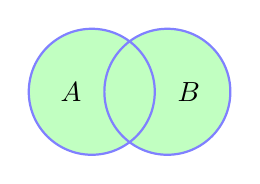
\begin{tikzpicture}[scale=.8]
  \filldraw[color=green!30!white,opacity=.8]
    (0,0) circle (1)
    (1.2,0)  circle (1);
  \draw[blue!50, thick]
    (0,0)  node[black,left] {$A$} circle (1)
    (1.2,0) node[black,right] {$B$} circle (1);
  %\filldraw[color=white,opacity=.4] (-.2,.8) rectangle (1.4,1.3);
  %\node at (.6,.8) [black,above] {$A\cup B$};
\end{tikzpicture}%
}{3cm}{}
\putthere{15.4cm}{-2.0cm}{%
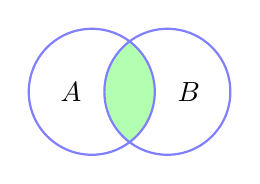
\begin{tikzpicture}[scale=.8]
  \begin{scope}
    \clip (0,0) circle (1);
    \filldraw[color=green!30!white,opacity=1.0] (1.2,0)  circle (1);
  \end{scope}
  \draw[blue!50, thick]
    (0,0)  node[black,left] {$A$} circle (1)
    (1.2,0) node[black,right] {$B$} circle (1);
%  \filldraw[color=white,opacity=.4] (-.2,.8) rectangle (1.4,1.3);
% \node at (.6,.8) [black,above] {$A\cap B$};
\end{tikzpicture}
}{3cm}{}
\putthere{15.4cm}{-3.9cm}{%
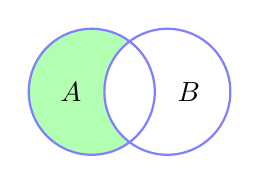
\begin{tikzpicture}[scale=.8]
  \filldraw[color=green!30!white,opacity=8.0] (0,0) circle (1);
  \filldraw[color=white] (1.2,0)  circle (1);
  \draw[blue!50, thick]
    (0,0)  node[black,left] {$A$} circle (1)
    (1.2,0) node[black,right] {$B$} circle (1);
%  \filldraw[color=white,opacity=.4] (-.2,.8) rectangle (1.4,1.3);
%  \node at (.6,.8) [black,above] {$A\setminus B$};
\end{tikzpicture}
}{3cm}{}
\выд{Объединение\/} множеств $A$ и $B$ %называется множество,
состоит из всех таких~$x$, которые принадле\-жат хотя бы одному
из множеств $A$ и~$B$ (то есть $x\in A$ или $x\in B$).
Обозначение:~\hbox{$A\cup B$}.\\
%\опр
\выд{Пересечение\/} множеств $A$ и $B$ %называется множество,
состоит из всех таких~$x$, что $x\in A$ и $x\in B$.
Обозначение:~$A\cap B$.\\
%\опр
\выд{Разность\/} множеств $A$ и $B$ %называется множество,
состоит из всех таких~$x$, что $x\in A$ и $x\notin B$.
Обозначение:~$A\setminus B$.\\
На рисунке справа объединение, пересечение и разность
показаны с помощью \выд{кругов Эйлера}.
\копр

\задача
%Пусть $A$~--- множество всех чётных чисел,
%$B$~--- множество всех чисел, делящихся на~3.
Пусть $A=\{2k+1 \mid k\in\Z\}$,
$B=\{3k \mid k\in\Z\}$. Найдите $A\cap B$ и $B\setminus A$.
\кзадача

%\задача
%Для каждых двух из следующих множеств укажите их пересечение, объединение
%и разность: множество равнобедренных треугольников; множество треугольников
%с углом $110^\circ$; множество треугольников со стороной 7;
%множество треугольников, у которых наименьший угол равен $30^\circ$.




\noindent
{\small
Чтобы доказать, что два множества $X$ и $Y$ равны, достаточно проверить,
что каждый элемент множества $X$ принадлежит множеству $Y$, и наоборот.
}

\ВосстановитьГраницы

\задача
Верно ли, что для любых множеств $A$, $B$ и $C$\\
\вСтрочку
\пункт $A\setminus(A\setminus B) = A\cap B$;
\пункт $A\cap B = A \Leftrightarrow A\subseteq B$;
\пункт $A\setminus B = C \Leftrightarrow A=B\cup C$?
%\пункт $A\setminus(B\setminus C) = (A\setminus B)\cup(A\cap C)$.
\кзадача




\задача
Докажите %\footnote{Указание: множества $X$ и $Y$ совпадают, если каждый
%элемент множества $X$ принадлежит множеству $Y$, и наоборот.}
для любых множеств $A$, $B$ и $C$:\\
\вСтрочку
\пункт $A\cap(B\cap C) = (A\cap B)\cap C$;
\пункт $A\cup(B\cap C) = (A\cup B)\cap(A\cup C)$;
\пункт $A\setminus(B\cap C) = (A\setminus B)\cup(A\setminus C)$.
\кзадача

\задача Посмотрите на диаграммы Эйлера-Венна ниже и запишите, каким множествам
соответствуют заштрихованные области. Для записи используйте
символы $\cup$, $\cap$, $\backslash$ и скобки.
\кзадача

 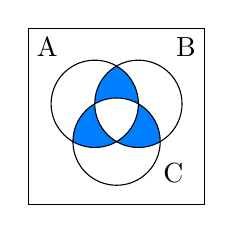
\begin{tikzpicture}[scale=0.16]

 \regionA{\mynocolor} \regionB{\mynocolor} \regionC{\mynocolor}
 \regionAB{\mycolor} \regionAC{\mycolor}\regionBC{\mycolor}
 \regionABC{\mynocolor}
   \draw (30:2) circle ({2*sqrt(3)});
   \draw (150:2) circle ({2*sqrt(3)});
   \draw (270:2) circle ({2*sqrt(3)});
   \draw (-5.5,5.5) node {A};
   \draw (4.5,-4.5) node {C};
   \draw (5.5,5.5) node {B};
    \draw (-7,-7) rectangle (7,7);

 \end{tikzpicture} \quad
  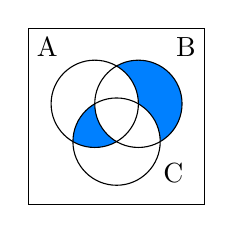
\begin{tikzpicture}[scale=0.16]

 \regionA{\mynocolor} \regionB{\mycolor} \regionC{\mynocolor}
 \regionAB{\mynocolor} \regionAC{\mycolor}\regionBC{\mynocolor}
 \regionABC{\mynocolor}
   \draw (30:2) circle ({2*sqrt(3)});
   \draw (150:2) circle ({2*sqrt(3)});
   \draw (270:2) circle ({2*sqrt(3)});
   \draw (-5.5,5.5) node {A};
   \draw (4.5,-4.5) node {C};
   \draw (5.5,5.5) node {B};
    \draw (-7,-7) rectangle (7,7);

 \end{tikzpicture} \quad 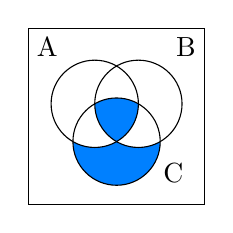
\begin{tikzpicture}[scale=0.16]

 \regionA{\mynocolor} \regionB{\mynocolor} \regionC{\mycolor}
 \regionAB{\mynocolor} \regionAC{\mynocolor}\regionBC{\mynocolor}
 \regionABC{\mycolor}
   \draw (30:2) circle ({2*sqrt(3)});
   \draw (150:2) circle ({2*sqrt(3)});
   \draw (270:2) circle ({2*sqrt(3)});
   \draw (-5.5,5.5) node {A};
   \draw (4.5,-4.5) node {C};
   \draw (5.5,5.5) node {B};
    \draw (-7,-7) rectangle (7,7);

 \end{tikzpicture}\quad 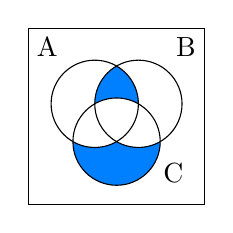
\begin{tikzpicture}[scale=0.16]

 \regionA{\mynocolor} \regionB{\mynocolor} \regionC{\mycolor}
 \regionAB{\mycolor} \regionAC{\mynocolor}\regionBC{\mynocolor}
 \regionABC{\mynocolor}
   \draw (30:2) circle ({2*sqrt(3)});
   \draw (150:2) circle ({2*sqrt(3)});
   \draw (270:2) circle ({2*sqrt(3)});
   \draw (-5.5,5.5) node {A};
   \draw (4.5,-4.5) node {C};
   \draw (5.5,5.5) node {B};
    \draw (-7,-7) rectangle (7,7);

 \end{tikzpicture} \quad 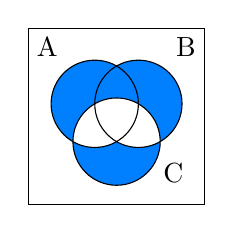
\begin{tikzpicture}[scale=0.16]

 \regionA{\mycolor} \regionB{\mycolor} \regionC{\mycolor}
 \regionAB{\mycolor} \regionAC{\mynocolor}\regionBC{\mynocolor}
 \regionABC{\mynocolor}
   \draw (30:2) circle ({2*sqrt(3)});
   \draw (150:2) circle ({2*sqrt(3)});
   \draw (270:2) circle ({2*sqrt(3)});
   \draw (-5.5,5.5) node {A};
   \draw (4.5,-4.5) node {C};
   \draw (5.5,5.5) node {B};
    \draw (-7,-7) rectangle (7,7);

 \end{tikzpicture} \quad 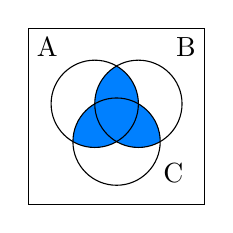
\begin{tikzpicture}[scale=0.16]

 \regionA{\mynocolor} \regionB{\mynocolor} \regionC{\mynocolor}
 \regionAB{\mycolor} \regionAC{\mycolor}\regionBC{\mycolor}
 \regionABC{\mycolor}
   \draw (30:2) circle ({2*sqrt(3)});
   \draw (150:2) circle ({2*sqrt(3)});
   \draw (270:2) circle ({2*sqrt(3)});
   \draw (-5.5,5.5) node {A};
   \draw (4.5,-4.5) node {C};
   \draw (5.5,5.5) node {B};
    \draw (-7,-7) rectangle (7,7);

 \end{tikzpicture}

\УстановитьГраницы{0pt}{3.5truecm}
\задача
\выд{Полуплоскость} --- это множество точек плоскости, лежащих
по одну сторону от некой прямой (в том числе и на самой этой прямой).
Какой многоугольник (с внутренностью) на рисунке нельзя
представить в виде пересечения нескольких полуплоскостей?
\кзадача
\ВосстановитьГраницы

\putthere{17.5cm}{.9cm}{%
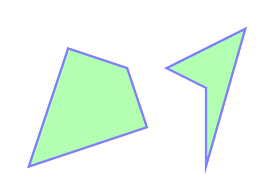
\begin{tikzpicture}[scale=.5]
  \filldraw[color=green!30!white,opacity=8.0, draw = blue!50, thick]
    (0,0) -- (3,1) -- (2.5,2.5) -- (1,3) -- cycle
    (3.5,2.5) -- (5.5,3.5) -- (4.5,0) -- (4.5,2) -- cycle;
\end{tikzpicture}%
}{1cm}{}

\vspace*{-.4cm}
\сзадача
\пункт Можно ли записать пересечение двух множеств, используя только разность и объединение?
\пункт Можно ли записать разность двух множеств, используя только
объединение и пересечение?
\кзадача

\раздел{Формула включений-исключений}

\задача
\пункт В НИИ 67 человек. Из них
47 знают английский, 35 --- немецкий, и 23 --- оба языка.
Сколько человек не знают ни английского, ни немецкого?
\пункт Пусть еще  польский
знают 20 человек, английский~и~поль\-с\-кий --- 12, немецкий и
польский --- 11, все три языка --- 5.
Сколько человек не знают ни одного из этих~языков?
%\пункт [Формула включений и исключений]
%Решите задачу в общем случае:
\кзадача

\задача В комнате площади 6 уложены три ковра площади 3 каждый (форма комнаты и ковров произвольная).
Докажите, что какие-то два из этих трёх ковров перекрываются по площади, не меньшей~1.
\кзадача

\задача
Пусть множества $A_1,\dots,A_n$ конечны. Докажите, что
\вСтрочку
\пункт  $|A_1\cup A_2|=|A_1|+|A_2|-|A_1\cap A_2|$.\\
\пункт
%Докажите, что
$|A_1\cup A_2\cup A_3|=|A_1|+|A_2|+|A_3|-|A_1\cap A_2|-|A_1\cap A_3|-
|A_2\cap A_3|+|A_1\cap A_2\cap A_3|$.\\
\спункт[Формула включений-исключений]
Выведите аналогичную формулу для $|A_1\cup A_2\cup\dots\cup A_n|$.
(Сравните с задачей 7, когда есть $n$ языков,
и для каждого набора языков известно, сколько человек знают все эти языки.)
\кзадача



% \задача
% В библиотеке $n$ книг и несколько читателей
% (каждый проч\"ел хотя бы одну книгу).~Про~лю\-бые $k$
% книг ($1\leq k\leq n$) известно, сколько читателей прочитало их все.
% Как найти общее число~читателей?
% \кзадача

\задача
В ряду $1+\ldots+1$ из 105 единиц
изменили знак на противоположный перед каждой третьей~единицей,
затем --- перед каждой пятой, а затем --- перед
каждой седьмой. Найдите значение полученного выражения.
\кзадача

\сзадача \вСтрочку
\пункт
На полке стоят 10 книг. Сколькими способами их можно переставить
так,~чтобы ни одна книга не осталась на месте?
\пункт А если на месте должны остаться ровно 3 книги?
\кзадача


%\сзадача
%Какое максимальное количество различных множеств можно получить
%из данных~$n$, используя операции $\setminus$, $\cup$ и $\cap\,$?
%\кзадача


%\vfill

\ЛичныйКондуит{0mm}{6mm}
% \GenXMLW

\end{document}

